%\documentclass[11pt,final]{fithesis}
\documentclass[11pt,draft,oneside]{fithesis}
\usepackage[plainpages=false, pdfpagelabels]{hyperref}
\usepackage[T1]{fontenc}  %aby boli pekne pismena
\usepackage[slovak]{babel}  %slovensky balik
\usepackage{longtable}     % pre vecsie tabulky
\usepackage{graphicx}
%\usepackage{a4wide}
\usepackage{lettrine}  %velke uvodne pismeno

\thesistitle{model nieco :D}
\thesissubtitle{Diplomov� pr�ca}
\thesisstudent{bc. Miroslav Ligas}
\thesiswoman{false}
\thesisfaculty{fi}
\thesislang{sk}
\thesisyear{jaro 2009}
\thesisadvisor{Mgr. Tom� Lud�k}


\begin{document}
\FrontMatter
\ThesisTitlePage

\begin{ThesisDeclaration}
\DeclarationText
\AdvisorName
\end{ThesisDeclaration}

\begin{ThesisThanks}
Dakujem za v�etko �o pre m�a urobili ...
\end{ThesisThanks}
......

\MainMatter
\tableofcontents
\chapter{�vod}
\label{chap:uvod}
S rie�en�m softv�rov�ch projektov vznikaj� r�zne probl�my, ktor� m��u vies� k zlyhaniu projektu. Tieto rizik� sa pri v�voji sna��me odstr�ni� zaveden�m metod�k, ktor� n�m napom�haj� uchopi� projekt, rozanalyzova� problematick� miesta a �o najlep�ie navrhn�� rie�enie. �iadna metodika n�m nezaist� splnite�nos� projektu ale jej pou�itie minimalizuje riziko krachu projektu. 

Najpou��vanej�ie modelovacie metodiky s��asnej doby s� ve�mi rozsiahle a siln� n�stroje. Definuj� ve�k� mno�stvo roli a zav�dzaj� komplexn� procesy, ��m dok�u zvl�da� ve�k� projekty. Vn�aj� t�m do v�voja ve�k� r�iu, ktor� projekt pom�ha lep�ie zvl�da� ale ho aj predl�uje. ��m je projekt men�� t�m je cite�nej�ia z�a� komplexnej metodiky. Opomenutie metod�k by zbavilo projekty v�etkej r�ie a u�etrilo by �as aj prostriedky, ale riziko, ktor� by vzniklo by mnohon�sobne prev��ilo �sporu. 

Pri modernom v�voji nie je preto rozumn� postupova� bez metodik pri akomko�vek v�voji. Napriek tomu sa naskytuje priestor na h�adanie nov�ch ciest pri ich rie�en�. Namiesto vyu��vania rozsiahlych pou��van�ch a overen�ch metodik sa treba zamera� na ich esenci�lne �asti. Na z�klade t�chto �ast� sa vybuduje �ahko zvl�dnute�n� a flexibiln� met�da. 

Mal� softv�rov� projekty s� v��inou sprac�van� neve�k�m po�tom pracovn�kov ako na strane v�voj�ra tak na strane klienta. Ukazuje sa tu preto miesto pre r�chlu a flexibiln� met�du, ktor� dok�e r�chlo produkova� funk�n� moduly a flexibilne reagova� na po�iadavky klienta. Cie�om tejto pr�ce je n�js� stanoven� met�du.

\section{�trukt�ra pr�ce}

Druh� kapitola pr�ce sa zaober� najpou��vanej��mi modelovac�mi n�strojmi, ktor� sa v s��asnosti pou��vaj� na zachytenie interakcie a stavu v danom syst�me. Podrobne sa  tu popisuje roz��ren� no mo�no nie tak notoricky zn�mi n�stroj na modelovanie firemn�ch procesov Business Process Modeling Notation (BPMN). Okrajovo sa spom�na aj Unified Modeling Language (UML). Popisovan� s� len niektor� prvky UML, s ktor�mi sa v pr�ci stretneme. \\

Tretia kapitola je venovan� metodik�m. Popisuje r�zne pr�stupy ako rie�i� budovanie syst�mu. Zaober� sa agiln�mi  metodikami, ktor� sa vyzna�uj� r�chlos�ou a flexibilitou. V kontraste k nim stoja tradi�n� �trukt�rovan� metodiky ako Unified Process (UP), ktor� stavaj� na definovan�ch postupoch a roliach. Podrobnej�ie sa venujeme najm� t�m, z�ktor�ch �erp�me in�pir�ciu pre zostavenie vlastnej met�dy. \\

�tvrt� kapitola zachyt�va hlavn� �as� pr�ce a to definovanie met�dy pre mal� softv�rov� projekty s vyu�it�m BPMN. V tejto kapitole sa uplat�uj� n�stroje a postupy definovan� v predch�dzaj�cich oddieloch.  Met�da je zostaven� zo zau��van�ch metod�k, z ktor�ch sa vyberaj� relevantn� �asti. Sp�ja sa v nej agiln� pr�stup a tradi�n� �trukt�rovan� metodiky. Metoda �erp� inspir�ciu z Business Driven Development (BDD) z dielne IBM. Na zachytenie po�iadavkov a identifik�ciu modulov v projektovanom syst�m pou��va hierarchiu BPMN diagramov. Jednotlive moduly s� n�sledne modelovan� za pomoci tradi�n�ch UML diagramov. \\

Z�vere�n� piata kapitola overuje vhodnos� definovanej met�dy. Z jej vyu�it�m je vytvoren� pr�padov� �t�dia popisuj�ca spr�vu vedeck�ho �asopisu. Pomocou uveden�ch n�strojov modeluje hierarchiu procesov prebiehaj�cich pri fungovan� spr�vy vedeck�ho �asopisu. Vo vzniknutej procesnej mape s� identifikovan� procesy, ktor� je mo�n� automatizova�. N�sledne s� ur�ene komponenty, ktor� s� pomocou UML modelovan� a na z�ver je na�rtnut� implement�cia. \\
\chapter{Pr�stupy vyvoja softv�ru}
\label{chap:metodmod}
obkec okolo metodik

\section{Inkrement�lny}
\label{sec:increm}

\section{Iitera�n�}
\label{sec:spiral}

\section{Agiln� metodiky}
\label{sec:agil}

\section{Business Driven Development}
\label{sec:bdd}

\section{Unified Process}
\label{sec:up}
\chapter{Unified Process}
\label{chap:up}
popis RUP omacky



\chapter{Bussines Process Modeling ???}
\label{chap:bpm}
obkec o BPM 

\chapter{Defin�cia a �pecifik�cia po�iadavkov}
\label{chap:defaspecifikaciapoziadavkov}
\section{�pecifik�cia po�iadavkov}

��elom syst�mu je zabezpe�i� virtu�lnu konferenciu. Webov� aplik�cia mus� ma� prvky redak�n�ho syst�mu, ktor� umo�nia administr�torovi upravova�, prid�va� a odobera� jej obsah. \\ \\

��elom aplik�cie bude zbieranie a sprostredkov�vanie �l�nkov vo forme virtu�lneho �asopisu. Aplik�cia bude zobrazova� na webov� rozhranie preh�ad z�kladn�ch inform�ci� o ka�dom �l�nku a to:
\begin{center}
\begin{itemize}
\item autora 
\item in�tit�ciu
\item n�zov
\item k���ov� slov�
\item anot�ciu
\item odkaz na pln� text v PDF form�te
\end{itemize}
\end{center}

Aplik�cia bude obsahova� vyh�ad�vanie v inform�ci�ch ulo�en�ch v datab�ze. Vyh�ad�vanie bude mo�n� pod�a z�kladn�ch inform�cii okrem anot�cie taktie� sa nebude vyh�ad�va� v samotnom texte �l�nkov.\\ \\

Ku ka�d�mu �l�nku bude diskusia kde budu m�c� u��vatelia vyjadri� svoj n�zor k �l�nku a bud� ma� mo�nos� reagova� na koment�re in�ch u��vate�ov. Diskusia bude rozvrstven� podla logickej n�v�znosti koment�rov.\\ \\

Aplik�cia bude rozli�ova� u��vate�ov, ktor� k nej budu pristupova�. Ka�d� u��vate�, ktor� sa neprihl�si bude ma� pr�vomoci neregistrovan�ho u��vate�a. Na registr�ciu bude k dispoz�cii formul�r na vytv�ranie nov�ch registorvan�ch u��vate�ov.\\ 

Administr�torsk� ��et bude pridelen� u��vate�ovi pri inicializa�nom spusten� webovej aplik�cie. Pr�padn� �al�ie administr�torsk� ��ty mus� vytv�ra� u� existuj�ci administr�tor.\\
Syst�m rozozn�va nasledovne u��vate�sk� skupiny:
\begin{itemize}
 \item[\textbf{Administr�tor}] - Administr�tor bude ma� mo�nos� manipulova� s obsahom str�nok, spravova� u��vate�ov a m� na starosti prvotn� konfigur�ciu. V spr�ve u��vate�ov bude potvrdzova� nov� �iadosti o registr�ciu, bude m�c� pozme�ova� �daje o u��vate�ovi, meni� ich role a blokova� ��ty.
\item[\textbf{Neregistrovan� u��vate�}] - Bude ma� mo�nos� prehliada� zoznam ulo�en�ch �l�nkov, m��e v nich vyh�ad�va� ale nem� pr�stup k pln�m textom �l�nkov.
\item[\textbf{Registrovan� u��vate�}] - Bude ma� v�etky pr�va neregistrovan�ho u��vate�a a naviac aj pr�stup k pln�m textom �l�nkov z ro�n�ka, pre ktor� zaplatil �lensk� poplatok. Taktie� bude m�c� za z�kladn� �lensk� poplatok vlo�i� jeden �l�nok. Bude si m�c� upravova� inform�cie v profile a meni� pristupov� heslo.
\item[\textbf{Redak�n� rada}] - Bude ma� mo�nos� stopn�� uverejnenie pr�spevku s od�vodnen�m jeho pozastavenia.
\item[\textbf{Recenzenti}] - Bud� ma� pr�stup k textom �l�nkov v upravite�nej podobe a k odovzdan�m �l�nkom maj� mo�nos� prid�va� recenzovan� verziu.
\end{itemize}

Aplik�cia bude obsahova� radu notifik�cii. Pri zalo�en� nov�ho ��tu bude zaslan� inform�cia administr�torovi so �iados�ou o jeho potvrdenie po overen� zaplatenia �lensk�ho poplatku.\\
Pri ka�dom vlo�en� nov�ho �l�nku registrovan�m u��vate�om bud� vybran� a obozn�men� o tomto �l�nku recenzenti, ktor�ch �lohou bude �l�nok recenzova�.\\
Registrovan� u��vatelia si m��u povoli� ozn�menie o nov�ch zverejnen�ch �l�nkoch cez mail a pre v�etk�ch u��vate�ov bude k dispoz�cii RSS zdroj. \\
Po dov�en� limitu na zostavenie ��sla �asopisu bude o tom informovan� redak�n� rada a administr�tor. \\ \\

Pravidelne bude sp���an� z�lohovanie datab�zy, ako aj ulo�en�ch pln�ch textov �l�nkov, ktor� bud� sl��i� na obnovenie d�t v pr�pade poruchy. Kompletn� z�lohy bud� ukladan� na predur�en� ulo�isko. \\ \\

Redak�n� prvky syst�mu umo�nia administr�torovi upravova� a dop��a� webov� rozhranie syst�mu. Bude ma� mo�nos� meni� logo port�lu, texty na str�nkach, prid�va� a zneplat�ova� nov� str�nky. \\
V�etky zmeny rozlo�enia str�nok sa bud� prejavova� v �trukt�re menu str�nky, ktor� bude najviac 2 �rov�ov�. Str�nky budu m�c� by� dopl�ovan� do ktorejko�vek �rovne menu.\\ \\

Webov� rozhranie bude umo��ova� zmenu vzh�adu pomocou dod�van�ch t�m. Aplik�cia bude vyhotoven� s jednou �tandardnou t�mou a s t�mou pre postihnut�ch. \\
T�ma sa bude pre registrovan�ch u��vate�ov uklada� do ich profilu.\\ \\

Nevyhnutn� konfigur�cia hotovej distrib�cie prebehne pri jeho prvom spusten�. Vytvori sa tu administr�torsk� konto a v�etky nevyhnutn� nastavenia aplik�cie. \\
Cel� nasleduj�ci beh syst�mu bude automaticky a v�etky pr�padne zmeny nastavenia a obsahu sa budu dia� cez webov� rozhranie administr�tora. \\ \\

Webov� rozhranie bude preh�adne a funkcion�lne, zamerane na r�chle dosiahnutie po�adovan�ch inform�ci�. Ka�d� str�nka mus� obsahova� tieto prvky:
\begin{center}
\begin{itemize}
\item logo a z�kladne �daje o organiz�cii zria�uj�cej virtu�lnu konferenciu
\item menu str�nok webov�ho rozhrania
\item ak je u��vate� neprihl�sen� -- mo�nos� prihl�si� sa do syst�mu
\item ak je u��vate� prihl�sen� -- meno u��vate�a a vo�bu na odhl�senie sa
\end{itemize}
\end{center}

Inform�cie o ulo�en�ch �l�nkoch sa budu zobrazova� do preh�adn�ho v�pisu obsahuj�ceho z�kladn� inform�cie. Z�znamy sa bud� zobrazova� pre aktu�lny rok. Star�ie ro�n�ky bud� ulo�en� v arch�ve. \\
Z�znamy pre aktu�lny ro�n�k budu chronologicky usporiadan� od najnov��ch po najstar�ie. Arch�v bude usporiadan� pod�a rokov a bude rovnako zoraden� ako aktu�lny ro�n�k. Parameter zora�ovanie bude m�c� u��vate� pozmeni� na meno, in�tit�ciu, n�zov a d�tum. Taktie� bude mo�nos� zmeni� vzostupnos� alebo zostupnos� usporiadania.\\
V pr�pade, �e z�znamov bude viac ako limit zobrazenia na jednu str�nku, zoznam sa stane viac stranov�m. U��vate� si bude m�c� zvoli� ko�ko z�znamov chce na jedne kr�t zobrazi�.\\ \\

Rozhranie vyh�ad�vania bude �o najjednoduch�ie. Bude poskytova� vo�by na ur�enie kateg�rie, v ktorej sa bude vyh�ad�va�:
\begin{center}
\begin{itemize}
\item meno, in�tit�cia, n�zov
\item k���ov� slov�
\item ro�n�k 
\end{itemize}
\end{center}

\begin{center}
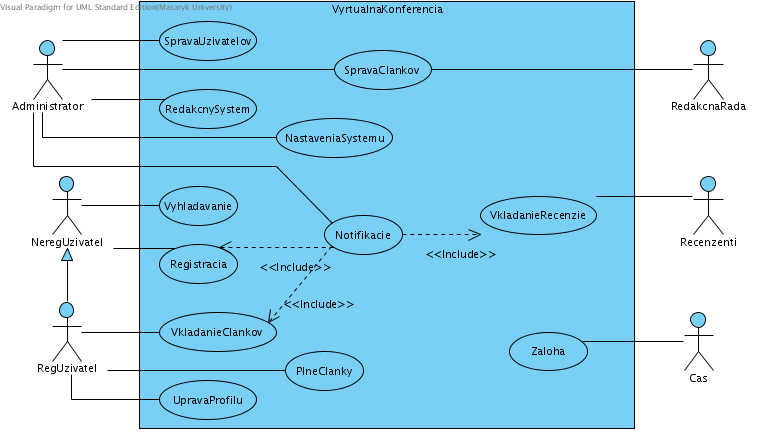
\includegraphics[width=\linewidth]{VyrtualnaKonferencia.png}
 % Use_Case_Diagram1.png: 742x436 pixel, 72dpi, 26.18x15.38 cm, bb=0 0 742 436
\textit{Use case diagram virtu�lnej konferencie.}
\end{center}

\chapter{Pr�padov� �t�dia v UP}
\label{chap:PsUP}
\section{Anal�za}
\section{N�vrh}

\chapter{Pr�padov� �t�dia v BPM}
\label{chap:PsBPM}
\section{Anal�za}
\section{N�vrh}


\chapter{Z�ver}
\label{chap:zaver}
V s��asnej dobe je v�voj softv�ru u� takmer nepredstavite�n� bez vyu�itia nejakej modelovacej met�dy, ktor� tento v�voj dok�e usmerni�, napom�c� z�skanie kvalitn�ho rie�enia probl�mu a rap�dne zv��i� �spe�nos� projektu. R�zne met�dy maj� rozdielne �pecifick� prvky a niektor� je potrebn� prisp�sobi� adekv�tnemu vyu�itiu a maximalizovaniu potenci�lu skr�vaj�ceho sa v nich. V�berom a pr�padnou �pravou postupu modelovania je zv��en� efekt�vnos� pr�ce, ur�chlen� v�voja a zn��en� n�klady na projekt. D�sledkom je dod�vanie kvalitn�ho softv�ru v dostupn�ch cenov�ch rel�ci�ch.

V�eobecne je hlavnou my�lienkou pou��vania metod�k u�ah�enie zvl�dnutia ve�k�ch projektov. Ke� v�ak aplikujeme rozsiahle a robustn� met�dy na mal�, jednoducho pochopite�n� a zvl�dnute�n� projekty, z�skavame zna�n� po�et �innost� nepos�vaj�cich projekt k r�chlemu koncu. Ve�k� po�et definovan�ch rol a modelov, ktor� musia by� vypracovan�, spoma�uje prechod k vlastn�mu produkovaniu syst�mu. Tento pr�stup ur�ite pon�ka monument�lny z�klad pre v�voj aplik�ci�, ale pre z�kazn�ka nemus� dod�va� rie�enia dostato�ne r�chlo. Pr�ve z�kazn�k potrebuje r�chle zavedenie IT rie�enia, aby zostala zachovan� jeho konkurencieschopnos�. Pri zd�havom dod�van� produktu m��e nasta� situ�cia, �e syst�m nesp��a r�chlo sa meniace po�iadavky klienta.

Na�tudovanie rozli�n�ch modelovac�ch met�d vyu��van�ch v minulosti a s��asnosti sl��ilo ako z�klad pre n�vrh met�dy umo��uj�cej efekt�vny v�voj mal�ch softv�rov�ch projektov. Popri pre�tudovan� modelov bolo cie�om tejto pr�ce aj obozn�menie sa s grafick�mi modelovac�mi n�strojmi, hlavne s Business Process Modeling Notation, sl��iacim na popisovanie firemn�ch procesov.

Navrhnut� met�da vyu��va BPMN diagramy na zachytenie po�iadaviek u��vate�a ako jeden zo vstupov do analytickej a v�vojovej �asti. Tieto diagramy s� intuit�vne pre z�kazn�ka, ktor� na z�klade nich m��e s analytikom diskutova� o dodanej funkcionalite realizovan�ho syst�mu. V�pr�pade, �e cie�ov� organiz�cia u� m� pop�san� �trukt�ru fungovania pomocou procesov, je t�m v�voj v�razne ur�chlen�.

Hlavn�m cie�om met�dy je r�chle dod�vanie kvalitn�ch IT rie�en� plniacich aktu�lne z�kazn�kove potreby. V navrhnutom postupe sa preto uplat�uj� my�lienky zachyten� v manifeste agiln�ho programovania. Vyzdvihovan� je spolupr�ca so z�kazn�kom a upravovanie n�vrhu a v�voja pod�a jeho predst�v. 

BPMN diagramy zachyt�vaj� funkcionalitu bud�ceho syst�mu. Charakterom pou�itia maj� prvky diagramov d�tov�ch tokov, ktor� boli v minulosti pou��van� pri n�vrhu softv�ru. Z�skava sa tak pomerne intuit�vny n�h�ad na fungovanie syst�mu, ktor� ke� spoj�me s diagramami tried pou��van�mi pri objektovo orientovanom n�vrhu, d�vaj� program�torovi jasn� rys budovan�ho syst�mu, ale tie� mu ponech�vaj� dostato�n� priestor na zapojenie svojej kreativity do realizovania v�sledn�ho rie�enia.

Navrhnut� met�da bola overen� pri vypracovan� informa�n�ho syst�mu pre spr�vu vedeck�ho �asopisu. Pod�a stanoven�ho postupu boli zachyten� po�iadavky na syst�m, ktor� boli preveden� na BPMN modely, a s ich pomocou boli vypracovan� diagramy pr�padov pou�itia a tried. Postupn� odvodzovanie diagramov prebehlo bez v���ch probl�mov. Z�skan� v�sledn� s�bor modelov popisuje statick� a dynamick� �trukt�ru produktu. 

Na �pln� overenie met�dy v�ak ch�ba realiz�cia navrhnut�ch modelov, ktor� v�ak nem��e by� preveden� tou istou osobou ako n�vrhov� �as�. Je potrebn� n�h�ad druhej, nezainteresovanej osoby, ktor� nem� so syst�mom sk�senosti a musela by sa preto spolieha� len na poskytnut� modely a komunik�ciu s n�vrh�rom. Overila by sa t�m miera zrozumite�nosti a mno�stvo inform�ci� poskytovan�ch modelmi.

\bibliographystyle{plain}  % bibliografick� styl 
\begin{thebibliography}{6}

%\bibitem{AEL}
%Microsoft MSDN Library (2007): \textit{About Event Logging}.
%On-line text: $<$http://msdn2.microsoft.com/en-us/library/aa363632.aspx$>$

\end{thebibliography}

\appendix 
\chapter{Pr�loha A}
%fsafas
\end{document}